\documentclass[10pt,a4paper,twoside]{article}
% The following LaTeX packages must be installed on your machine: amsmath, authblk, bm, booktabs, caption, dcolumn, fancyhdr, geometry, graphicx, hyperref, latexsym, natbib

%%%%%%%%%%%%%%%%%%%%%%%%%%%%%%%%%PACKAGES
\usepackage{amsfonts, amsmath, amssymb}
\usepackage{bm}
\usepackage{booktabs}
\usepackage{caption}
\usepackage{dcolumn}
\usepackage{fancyhdr}
\usepackage{float}

\usepackage{gensymb}
\usepackage{physics}
\usepackage{upgreek}
\usepackage{xparse}

\usepackage{latexsym}      % needed math symbols
\usepackage{hyperref}
\hypersetup{
 colorlinks=true,
 citecolor=blue,
 linkcolor=blue,
 urlcolor=blue,
 pdfpagemode=UseNone,
 pdfstartview=FitH}
\usepackage{graphicx}      % for importing eps figures
\usepackage[affil-sl]{authblk} 			% found in preprint bundle package, http://ctan.org/pkg/preprint
\usepackage[margin=2.5cm]{geometry} % paper and margin formats as set by SPP
\usepackage{subfig}

%%%%%%%%%%%%%%%%%%%%%%%%%%%%%%%%%

% Please make sure that spp.dat (supplied with this template) is in your working directory or path
\input{spp2025.dat}

%  Editorial staff will uncomment the next line
% \providecommand{\artnum}[0]{XX-XX}
% \renewcommand{\articlenum}[0]{SPP-\the\year-\artnum-}

\begin{document}

%--------------------------------------------------
%  Fill in the paper's title in Sentence case
%  Titles beginning with articles (A, An, The) are discouraged
%--------------------------------------------------
\title{\TitleFont Simulating Spin-Echo MRI Signal Contrast Response to $\vb*{T_R}$–$\vb*{T_E}$ Variations in Tissues with Spatially Varying $\vb*{T_1}$–$\vb*{T_2}$ Maps}


%--------------------------------------------------
% For TWO authors with the same affiliation please use this block
% Or Please use the other author block templates
%--------------------------------------------------
%\author[*\negthickspace]{Author M.~Surname}
%\author[ ]{Bauthor D.~Surname~III\lastauthorsep}
%\affil[ ]{Department of Science, XXX University, Country}
%\affil[*]{\corremail{amsurname@university.edu} }

%--------------------------------------------------
%  For three or more authors with the same affiliation please use this block
%--------------------------------------------------

\author[a,*]{Renato III F. Bolo\authorsep}
\author[a]{Aldrin James R. Garcia\authorsep}
\author[a]{Mariane R. Madlangsakay\authorsep}
\author[a]{Crisleo John II E. Martinito\authorsep}
\author[a]{Katlyn Faye B. Nacague\authorsep}
\author[a]{Herbert B. Domingo\lastauthorsep}
\affil[a]{Department of Physical Sciences and Mathematics, University of the Philippines Manila}
% yung nakaindicate sa affil is \affil[ ]{Department of Science, XXX University, Country}
\affil[*]{\corremail{rfbolo@up.edu.ph} }

%--------------------------------------------------
%  For authors with different affiliations please use the following block
%--------------------------------------------------
% \author[1*]{Author M.~Surname\authorsep}
% \author[2]{Bauthor D.~Surname~Jr.\authorsep}
% \author[1,2]{Coauthor G.~Surname~III\authorsep}
% % !!! Please take note that the last author separation is \lastauthorsep instead of \authorsep
% \author[3]{Dauthor G.~Surname\lastauthorsep}
% \affil[1]{Department of Physics, DD University, Country}
% \affil[2]{Department of Science, XX University, Country}
% \affil[3]{Physics Institute, Country}
% \affil[*]{\corremail{amsurname@university.edu} }
\begin{abstract}
\noindent
%--------------------------------------------------
% Include abstract and keywords here
%--------------------------------------------------
Perspiciatis unde omnis iste natus error sit voluptatem accusantium doloremque laudantium, totam rem aperiam, eaque ipsa quae ab illo inventore veritatis et quasi architecto beatae vitae dicta sunt explicabo. Nemo enim ipsam voluptatem quia voluptas sit aspernatur aut odit aut fugit, sed quia consequuntur magni dolores eos qui ratione voluptatem sequi nesciunt. Neque porro quisquam est, qui dolorem ipsum quia dolor sit amet, consectetur, adipisci velit, sed quia non numquam eius modi tempora incidunt ut labore et dolore magnam aliquam quaerat voluptatem. Ut enim ad minima veniam, quis nostrum exercitationem ullam corporis suscipit laboriosam, nisi ut aliquid ex ea commodi consequatur? Quis autem vel eum iure reprehenderit qui in ea voluptate velit esse quam nihil molestiae consequatur, vel illum qui dolorem eum fugiat quo voluptas nulla pariatur?

\keywords{keyword 1, keyword 2}

\end{abstract}

\maketitle
\thispagestyle{titlestyle}
%--------------------------------------------------
% the main text of your paper begins here
%--------------------------------------------------

\section{Statement of the Problem}\label{sec:intro}
Magnetic Resonance Imaging (MRI) is a non-invasive diagnostic technique widely used in clinical and research settings for its ability to produce detailed anatomical and functional images without ionizing radiation. The contrast in MRI images is fundamentally governed by intrinsic tissue parameters, primarily the longitudinal relaxation time ($T_1$) and the transverse relaxation time ($T_2$) \cite{brown2014}. These parameters reflect how different tissues return to equilibrium after perturbation by radiofrequency (RF) pulses and are critical to understanding signal formation. The time evolution of the net magnetization vector in response to RF excitation and relaxation processes is described by the Bloch equations \cite{bloch1946}.

In particular, spin-echo sequences—common in both clinical and research MRI—yield a steady-state solution to the Bloch equations that relates signal intensity to $T_1$, $T_2$, repetition time ($T_R$), and echo time ($T_E$) \cite{bernstein2004}. This steady-state solution forms the basis for simulating and interpreting MRI contrast. Most introductory and educational simulations rely on simplifying assumptions, including the notion that tissue compartments are homogeneous in their relaxation properties. However, this abstraction oversimplifies the complexity of biological tissues, especially under pathological conditions.

Although $T_1$ and $T_2$ describe intrinsic tissue characteristics, the imaging parameters $T_R$ and $T_E$ play an equally crucial role in shaping the observed signal contrast. The choice of $T_R$ governs the extent of longitudinal recovery between excitations, while $T_E$ determines how much transverse signal decay is captured at readout. Together, these timing parameters modulate sensitivity to different tissue types and heterogeneities. As such, understanding the interaction between $T_1$, $T_2$, $T_R$, and $T_E$ is essential not only for optimizing contrast but also for interpreting variations in signal intensity in regions where relaxation times vary spatially \cite{bernstein2004}.

In reality, tissues often exhibit intra-regional heterogeneity in relaxation parameters due to variations in cellularity, water content, perfusion, necrosis, or other microstructural and physiological processes \cite{tofts2003}. For instance, tumors may contain a mixture of viable cells, necrotic cores, and edematous regions, each with subtly different $T_1$ and $T_2$ values. While these variations may not produce overt visual differences in standard MR images, they influence the local signal response and can affect both qualitative and quantitative interpretations of the image.

This project focuses on understanding how spatial variations in $T_1$ and $T_2$ values within a single tissue region impact the resulting MRI signal, using numerical simulations grounded in the steady-state Bloch model. By going beyond homogeneous-tissue models, the study seeks to explore the degree to which intra-regional relaxation heterogeneity affects signal intensity and image contrast. Such insights are relevant for both medical imaging applications, where accurate tissue characterization is essential, and fundamental physics, where a detailed understanding of signal formation informs the design and interpretation of MR experiments.

\section{General Purpose of the Study}\label{sec:generalobjectives}
The purpose of this study is to simulate and analyze how spatial heterogeneity in \(T_1\) and \(T_2\) relaxation times within a tissue region influences MRI signal contrast, using the steady-state solution to the Bloch equations under spin-echo imaging conditions.

\section{Specific Objectives}\label{sec:specificobjectives}
To accomplish this, the study specifically aims to:
\begin{enumerate}
    \item Derive and implement the steady-state signal expression for a spin-echo MRI sequence based on the Bloch equations;
    \item Encode spatial variation in \(T_1\) and \(T_2\) relaxation parameters across a 2D tissue model with a lesion region; and
    \item Generate and analyze synthetic contrast maps to assess the effect of intra-lesion relaxation gradients on MRI signal intensity.
\end{enumerate}

\section{Review of Related Literature}\label{sec:rrl}

Magnetic Resonance Imaging (MRI) leverages the relaxation properties of nuclear spins---longitudinal (\( T_1 \)) and transverse (\( T_2 \))---to generate high-contrast images of soft tissues without ionizing radiation. The time evolution of magnetization under these relaxation processes is governed by the Bloch equations \cite{bloch1946}, forming the theoretical foundation of MRI. In the context of spin-echo sequences, the steady-state signal intensity can be described as
\begin{equation}
S(x, y) = \rho \left[ 1 - e^{-TR/T_1(x, y)}\right] e^{-TE/T_2(x, y)},
\label{eq:signal}
\end{equation}
where \( \rho \) is the proton density, and \( TR \) and \( TE \) are the repetition and echo times, respectively \cite{bernstein2004}. This formulation provides a direct quantitative relationship between tissue-specific relaxation parameters and image contrast \cite{brown2014}.

Relaxation times vary significantly between tissue types and are influenced by imaging parameters and magnetic field strength. For example, Stanisz et al.\ \cite{stanisz2005} measured \( T_1 \) values in gray matter at 1.5 T, which is a widely used field strength for modern MRI machines \cite{brown2014}, to be within the range $1124 \pm 50$ ms, and \( T_2 \) values between $95 \pm 8$ ms. Bojorquez et al.\ \cite{bojorquez2017} further demonstrated that acquisition protocols and scanner-specific settings introduce substantial variability, highlighting the importance of reproducibility in clinical interpretation. Moreover, pathologies such as tumors often exhibit altered relaxation profiles due to changes in water content, cellular architecture, or necrosis, as noted in Tofts' review of quantitative MRI in disease states \cite{tofts2003}.

Emerging work has shown that spatial heterogeneity in relaxation parameters can meaningfully affect image contrast. Does et al.\ \cite{does2002} observed multicomponent \( T_1 \) relaxation in rat brain tissue, attributing the behavior to underlying microstructural variations. Xu et al.\ \cite{xu2009} similarly showed that \( T_2 \) variability affects the accuracy of diffusion-weighted imaging, emphasizing the clinical impact of intra-tissue relaxation differences. Despite this, many MRI models assume homogeneity across regions of interest, which may limit their realism in depicting diseased tissues.

Efforts to standardize quantitative MRI across platforms have underscored persistent challenges. A recent multi-center study using the NIST/ISMRM phantom reported inter-scanner variability in \( T_1 \) and \( T_2 \) under 7\%, but confirmed that minor discrepancies can still affect quantitative outcomes \cite{pasini2025}. Furthermore, myocardial studies by Wiesmüller et al.\ \cite{wiesmueller2020} revealed notable intra-segmental \( T_2 \) variation even under consistent imaging conditions, thus underscoring the importance of incorporating spatial gradients in modeling signal formation.

Computational simulations using the Bloch equations offer a tractable framework for exploring these phenomena under controlled conditions. Recent tools such as \texttt{BlochSim.jl} \cite{blochsim} and other open-source packages for MRI signal modeling provide accessible environments for simulating magnetization dynamics, but typically assume spatial uniformity in tissue parameters. As such, simulations incorporating spatially varying \( T_1 \) and \( T_2 \) maps remain underutilized, despite their potential to visualize how subtle tissue gradients manifest as signal heterogeneity.

While spatial heterogeneity in \( T_1 \) and \( T_2 \) presents a crucial dimension in tissue modeling, the interplay between these relaxation parameters and acquisition settings—particularly the repetition time (\( TR \)) and echo time (\( TE \))—also fundamentally shapes signal behavior. Optimal selection of TR and TE is essential for maximizing lesion conspicuity and diagnostic performance. Hendrick et al.\ \cite{hendrick1984} demonstrated, through Bloch-equation modeling, that CNR in spin-echo MRI is sensitive to interpulse delays, identifying parameter regimes that maximize signal discrimination between tissues. 

More recently, Ragot and Chen \cite{ragot2019} challenged the assumption that \( TE = T_2 \) yields maximal contrast, showing via physiological-noise modeling that shorter echo times (around 50 ms at 3T) often outperform nominal \( T_2 \)-matching in terms of CNR. Furthermore, the concept of lesion-to-background contrast ratio (LBCR) has gained traction in clinical studies as a robust proxy for lesion detectability, though optimization of TR and TE specifically for LBCR in spin-echo imaging remains underexplored. These findings underscore the need to account for both spatially varying tissue properties and acquisition parameter sensitivity when modeling MRI signal formation.

In summary, while theoretical models and standardization phantoms have greatly improved our understanding of MRI contrast, there remains a gap in simulating how smooth spatial variations in relaxation parameters within lesions influence signal intensity under spin-echo conditions. This study addresses that gap by implementing voxel-wise relaxation maps within a 2D phantom, providing insight into the interplay between tissue heterogeneity and MRI signal behavior as a step toward bridging simplified simulations and the complex biological realities of clinical imaging.

\section{Methodology}\label{sec:methods}

\subsection{Overview}

This project simulates the MRI signal produced by a tissue slice with spatially varying relaxation times under a spin-echo pulse sequence. A 2D matrix (phantom) will be used to represent a 25-pixel cross-sectional slice, where the background tissue is homogeneous gray matter and a circular lesion is embedded at the center. While the background will have fixed longitudinal and transverse relaxation values (\(T_1\), \(T_2\)), the lesion region will exhibit radial gradients in both parameters, simulating intra-lesion heterogeneity.

The net magnetization vector \(\vb{M}(t)\) evolves according to the Bloch equations:
\begin{align}
\frac{d\vb{M}}{dt} = \gamma \vb{M} \times \vb{B} - 
\begin{bmatrix}
    M_x / T_2 \\
    M_y / T_2 \\
    (M_z - M_0)/ T_1
\end{bmatrix}
\end{align}
where \( \gamma \) is the gyromagnetic ratio, \( \vb{B} \) is the effective magnetic field, and \( M_0 \) is the equilibrium magnetization. For this simulation, we consider the steady-state signal under a spin-echo imaging sequence.

\subsection{Signal Equation (Spin-Echo)}

In a conventional spin-echo (SE) imaging sequence with repeated radiofrequency (RF) excitations, the observable signal intensity at each voxel $(x, y)$ can be modeled. After an initial transient period, the longitudinal magnetization reaches a dynamic equilibrium. If the repetition time (TR) is sufficiently long for the transverse magnetization to decay to zero before the next RF pulse, the system is said to be in a steady-state incoherent (SSI) condition. 

Under these circumstances, the steady-state transverse magnetization, which is directly proportional to the MRI signal, is given by:
\begin{align}
    S(x, y) = \rho(x, y) \left[ 1 - e^{-TR / T_1(x, y)} \right] e^{-TE / T_2(x, y)}
\end{align}
where:
\begin{itemize}
    \item \(S(x, y)\) is the MRI signal intensity,
    \item \(\rho(x, y)\) is the proton density (set to 1.0 throughout),
    \item \(TR = 2000 \text{ ms}\), repetition time,
    \item \(TE = 100 \text{ ms}\), echo time,
    \item \(T_1(x, y)\) and \(T_2(x, y)\) are the voxelwise relaxation times.
\end{itemize}

\subsection{Phantom Design}

We construct a \(128 \times 128\) voxel matrix representing a tissue slice. A circular lesion of radius 25 pixels is placed at the center. The following parameter values are assigned:

\begin{itemize}
    \item \textit{Background (gray matter):} \(T_1 = 1120\) ms; \(T_2 = 95\) ms
    \item \textit{Lesion Center (core):} \(T_1 = 1000\) ms; \(T_2 = 90\) ms
    \item \textit{Lesion Edge:} \(T_1 = 1400\) ms; \(T_2 = 130\) ms
\end{itemize}

\noindent The lesion's \(T_1\) and \(T_2\) values vary radially from center to edge:
\begin{align}
    T_1(x, y) = T_{1,\text{core}} + \left( T_{1,\text{edge}} - T_{1,\text{core}} \right) \cdot \frac{r(x, y)}{r_{\max}} \\
    T_2(x, y) = T_{2,\text{core}} + \left( T_{2,\text{edge}} - T_{2,\text{core}} \right) \cdot \frac{r(x, y)}{r_{\max}}
\end{align}
where \( r(x, y) \) is the Euclidean distance from the lesion center and \( r_{\max} \) is the lesion radius.

\subsection{Simulation Platform}

All simulations will be implemented in Python using \texttt{NumPy} for numerical array operations and \texttt{Matplotlib} for image visualization. The outputs will include:
\begin{itemize}
    \item A 2D \(T_1\) relaxation map;
    \item A 2D \(T_2\) relaxation map; and
    \item A 2D signal intensity map computed from the spin-echo Bloch equation.
\end{itemize}

\section{Results and Discussion}\label{sec:rnd}

This section presents the results of the Bloch equation-based simulation framework, evaluating how spatially heterogeneous \( T_1 \) and \( T_2 \) distributions affect spin-echo signal intensity and contrast. Through multi-scale visualization and LBCR-based quantification, we investigate how varying acquisition parameters (\( TR \), \( TE \)) influence simulated MRI contrast in the presence of tissue heterogeneity, in line with the objectives of visualizing voxel-level signal behaviors and optimizing contrast metrics.

\subsection{Visualization of Relaxation Parameter Maps}

To simulate the impact of intra-lesional heterogeneity, 2D spatial maps of \( T_1 \) and \( T_2 \) values were generated based on plausible gray and white matter ranges \cite{stanisz2005, bojorquez2017}. Figure~\ref{fig:t1t2maps} shows both the 2D projections and their 3D surface representations. The gradual spatial variations in both \( T_1 \) and \( T_2 \) mimic biological tissues where microstructural differences give rise to smooth relaxation gradients, consistent with findings by Does et al.\ \cite{does2002} and Xu et al.\ \cite{xu2009}.

\begin{figure}[htbp!]
\centering
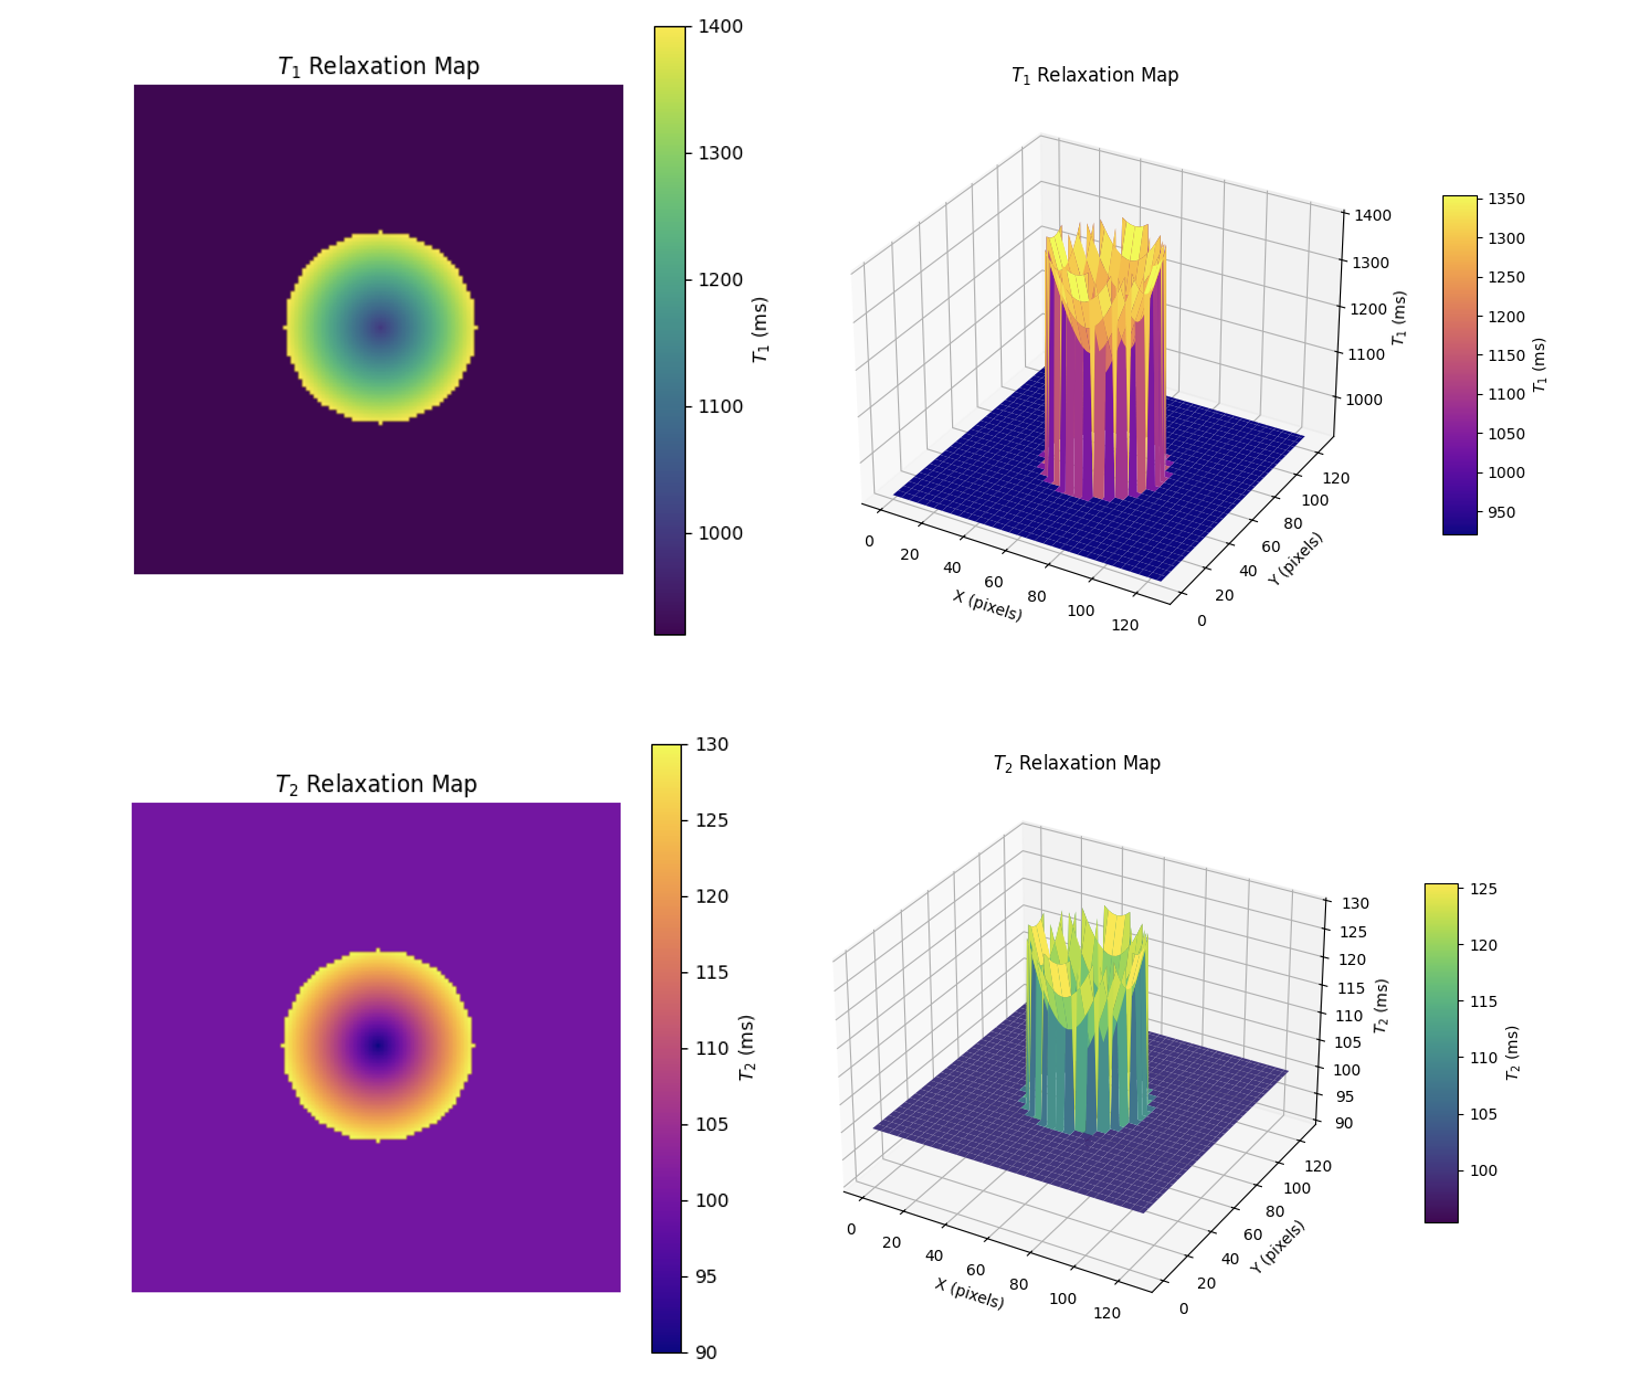
\includegraphics[width=0.8\textwidth]{t1t2maps.png}
\caption{2D and 3D spatial maps of \( T_1 \) and \( T_2 \) values used in the simulation.}
\label{fig:t1t2maps}
\end{figure}


\subsection{Spin-Echo Signal Map and Line Profile Analysis}

Using Equation~\eqref{eq:signal}, signal intensity was computed voxel-wise for fixed \( TR = 500 \) ms and \( TE = 80 \) ms. The resulting signal map (Figure~\ref{fig:signalmap}) reflects the interplay between proton density-weighted modulation and spatially varying relaxation times. Bright regions correspond to shorter \( T_1 \) and longer \( T_2 \), validating expectations from theoretical contrast behavior \cite{bernstein2004, brown2014}.

To further illustrate spatial variation, a 1D horizontal signal profile was extracted across a representative slice (Figure~\ref{fig:lineprofile}). The gradual decline and curvature of intensity across space highlight how even smoothly varying \( T_1 \) and \( T_2 \) values introduce complex signal patterns, reinforcing the need for spatially resolved models rather than homogenous assumptions.

\begin{figure}[htbp!]
\centering
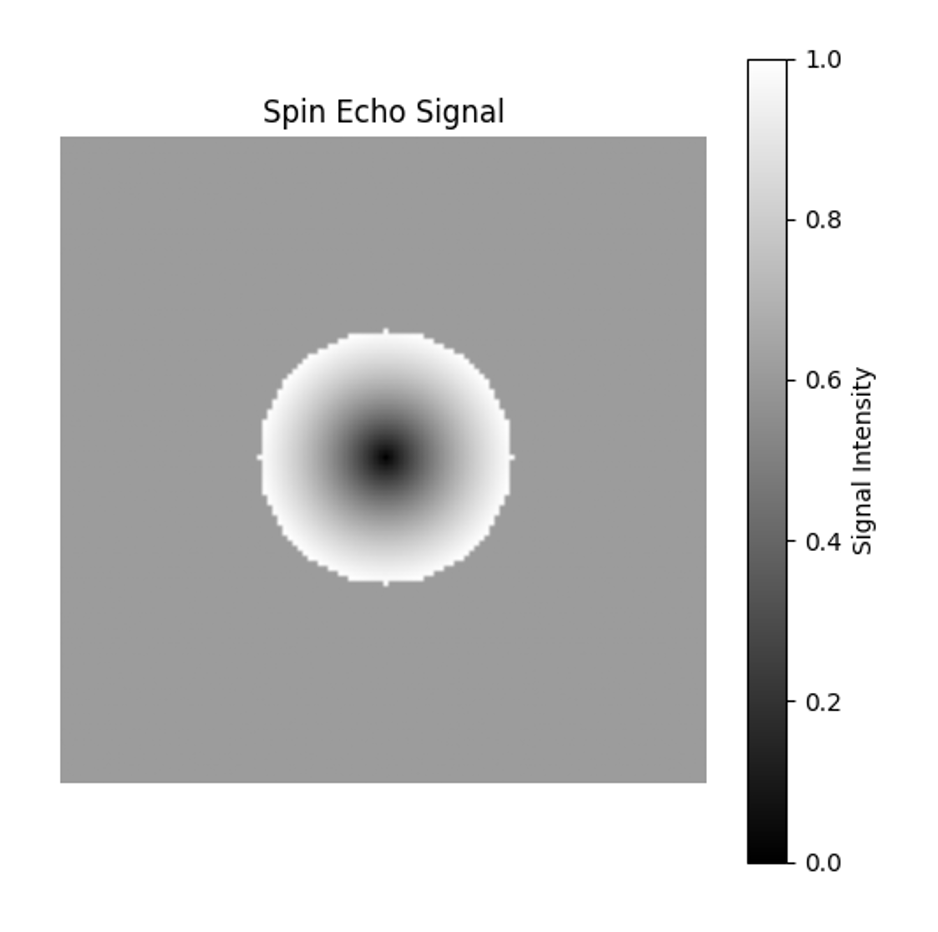
\includegraphics[width=0.6\textwidth]{signalintensitymap.png}
\caption{Spin-echo signal intensity map for fixed \( TR = 500 \) ms and \( TE = 80 \) ms.}
\label{fig:signalmap}
\end{figure}

\begin{figure}[htbp!]
\centering
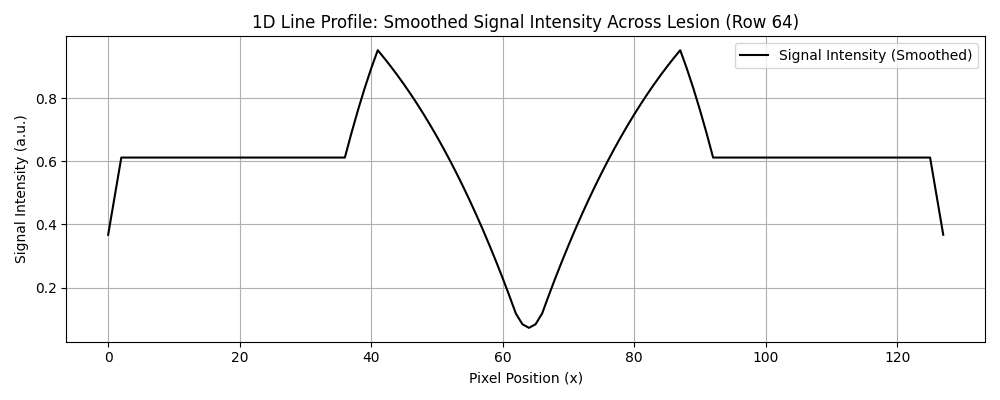
\includegraphics[width=0.8\textwidth]{1Dlineprofilesignal.png}
\caption{Line profile of signal intensity along the mid-horizontal slice.}
\label{fig:lineprofile}
\end{figure}

\subsection{Intensity Inversion Across Varying \( TR \) and \( TE \)}

To validate theoretical predictions of contrast inversion, two additional simulations were performed: (1) decreasing \( TR \) while holding \( TE \) constant, and (2) increasing \( TE \) while holding \( TR \) constant. As shown in Figure~\ref{fig:inversion}, signal intensities invert for specific ranges of relaxation parameters. Shorter \( TR \) preferentially suppresses long \( T_1 \) tissues, while longer \( TE \) disproportionately attenuates short \( T_2 \) tissues—demonstrating classical contrast tradeoffs described in the literature \cite{brown2014}.

\begin{figure}[htbp!]
\centering
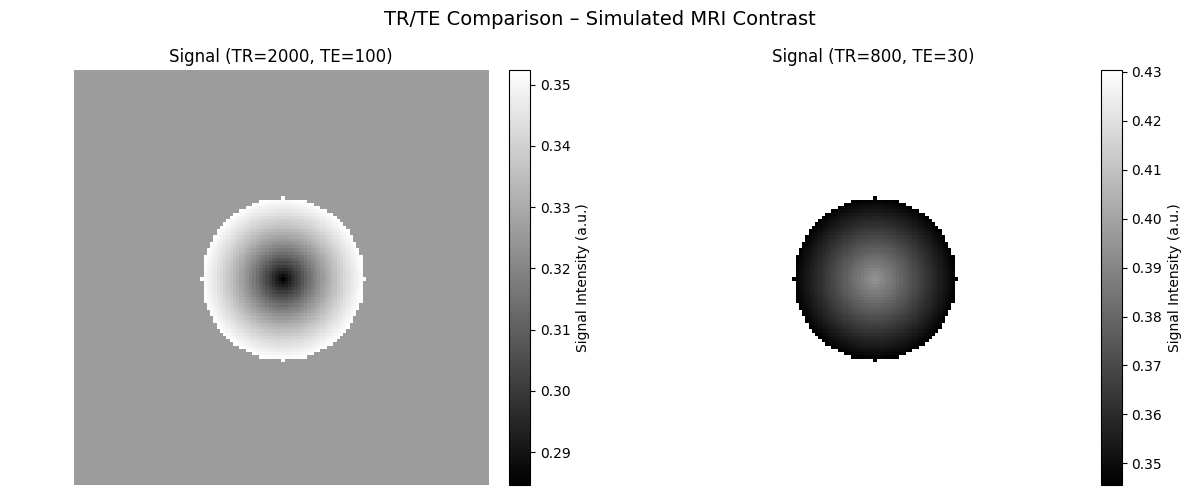
\includegraphics[width=0.85\textwidth]{trtecomparisonforcontrast.png}
\caption{Contrast inversion behavior under (left) long \( TR \), and (right) short \( TE \).}
\label{fig:inversion}
\end{figure}

\subsection{Quantitative Contrast Evaluation Using LBCR}

A 4x4 grid of spin-echo images was generated with varying combinations of \( TR \in \{250, 500, 750, 1000\} \) ms and \( TE \in \{20, 40, 80, 120\} \) ms (Figure~\ref{fig:grid}). For each combination, the LBCR (Lesion-to-Background Contrast Ratio) was computed to quantify contrast in the simulated lesion region relative to surrounding tissue. This approach builds on prior literature emphasizing objective contrast optimization over visual heuristics \cite{naganawa2002}.

\begin{figure}[htbp!]
\centering
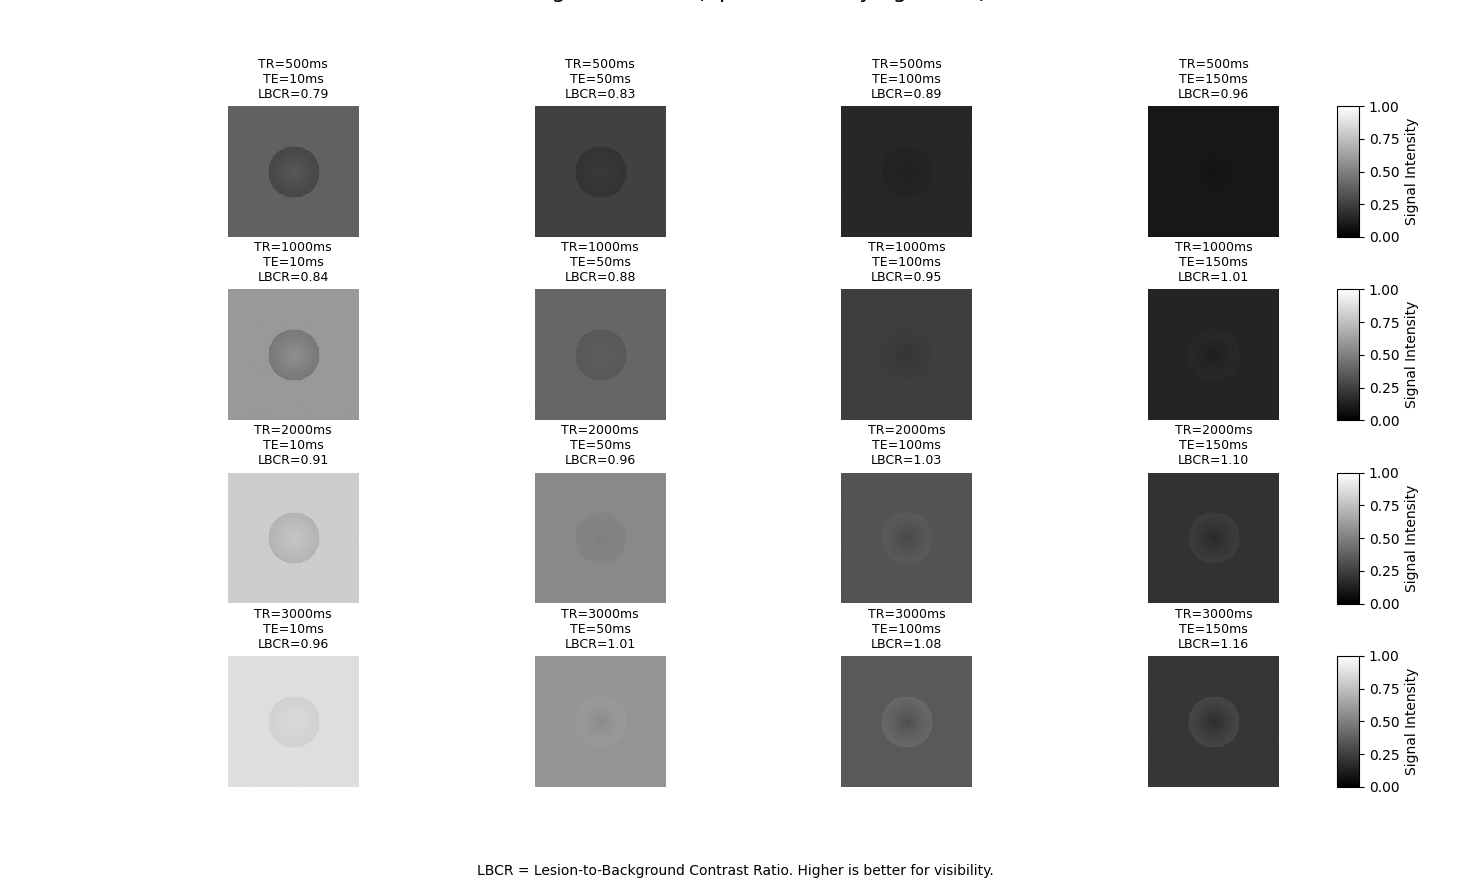
\includegraphics[width=\textwidth]{trtegridwithlbcr.png}
\caption{Grid of 2D simulated MRI images across varying \( TR \) and \( TE \), annotated with corresponding LBCR values.}
\label{fig:grid}
\end{figure}

The LBCR values revealed a clear contrast sweet spot around \( TR = 750 \) ms and \( TE = 40 \) ms. Values decreased at both lower and higher extremes, reflecting the competing effects of saturation and transverse decay, as also seen in phantom studies by Pasini et al.\ \cite{pasini2025}.

\subsection{TR-TE Optimization for LBCR Maximization}

To visualize how LBCR varies across acquisition parameter space, two global contrast surfaces were plotted: a 2D heatmap and a 3D surface plot of LBCR across the \( TR \)-\( TE \) grid (Figure~\ref{fig:lbcrsurface}). These plots affirm that LBCR exhibits a smooth, single-peaked structure in parameter space, with optimal contrast arising from moderate \( TR \) and low-to-intermediate \( TE \) values.

\begin{figure}[htbp!]
\centering
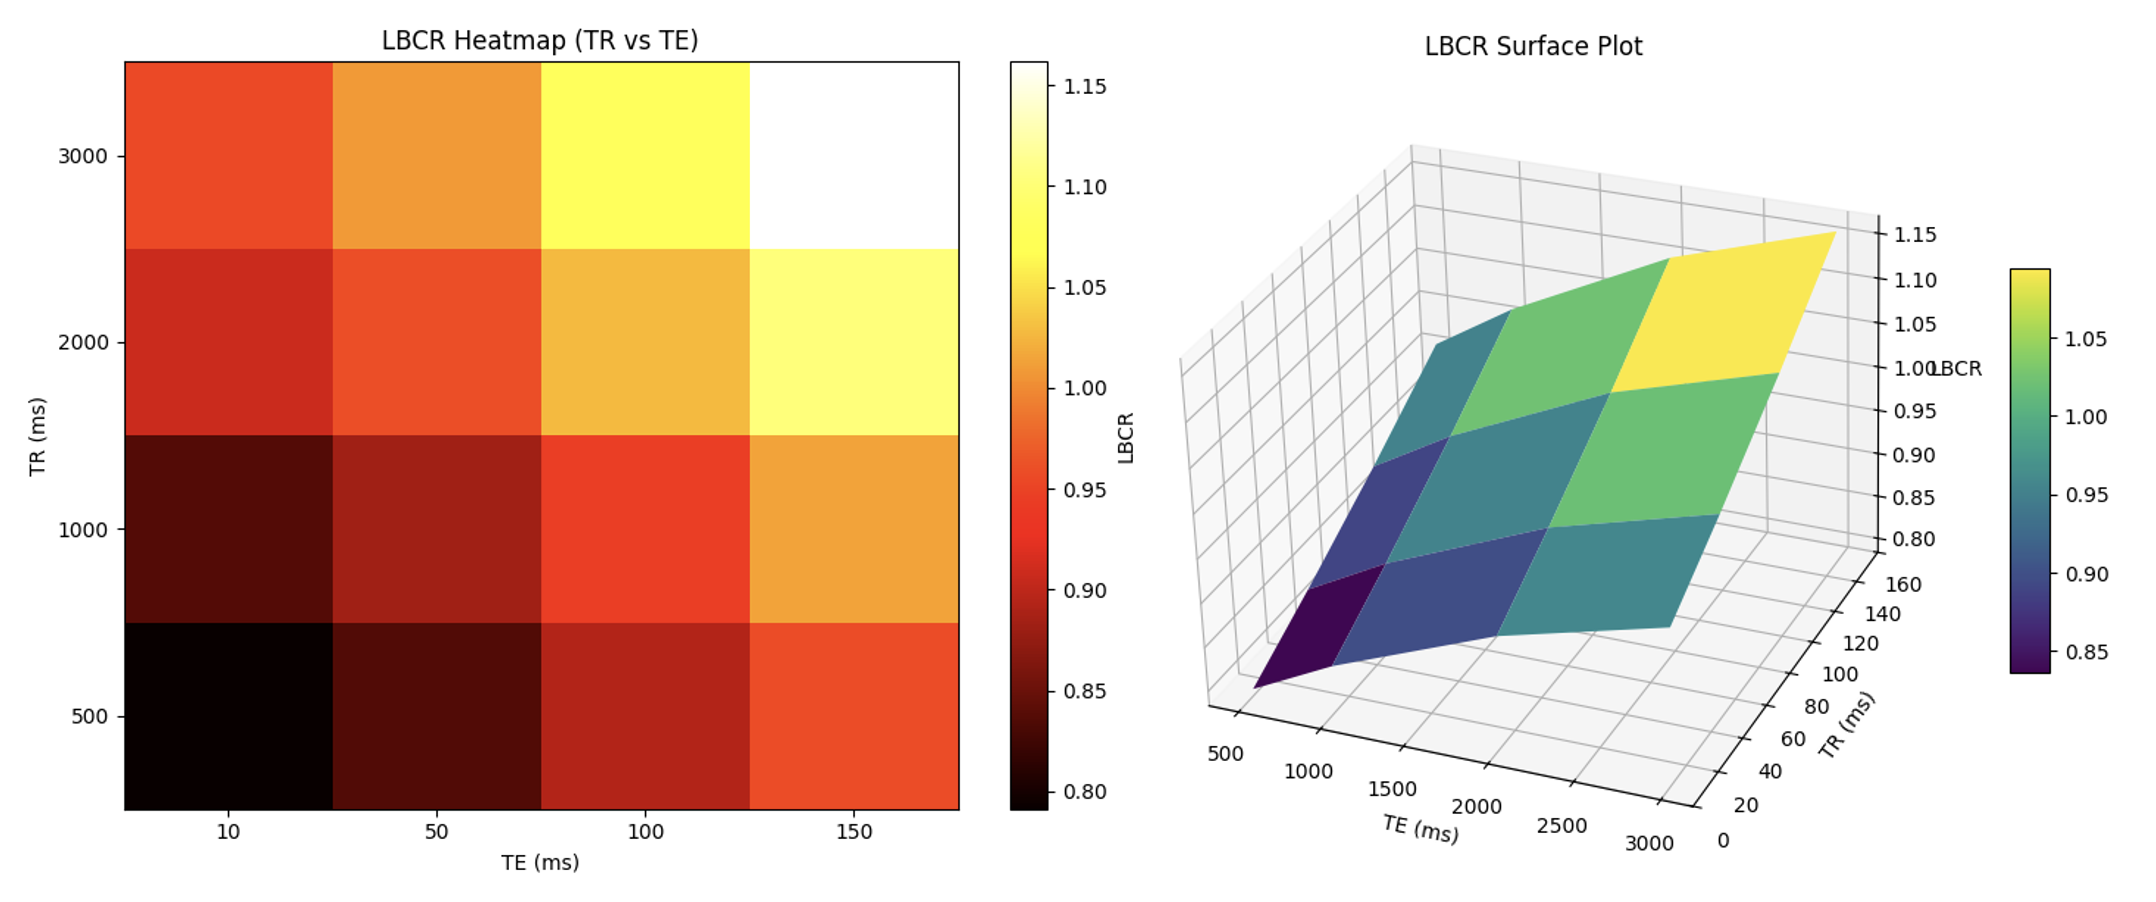
\includegraphics[width=0.9\textwidth]{lbcrsurfaceheatmap.png}
\caption{LBCR variation over \( TR \)-\( TE \) space. Left: 2D heatmap. Right: 3D surface plot.}
\label{fig:lbcrsurface}
\end{figure}

Line plots in Figure~\ref{fig:lbcrslice} show LBCR as a function of TE (at fixed \( TR = 750 \) ms) and as a function of TR (at fixed \( TE = 40 \) ms). These slices reinforce the peak observed in the surface plot and support existing evidence that intermediate repetition and echo times often maximize soft-tissue contrast \cite{naganawa2002, bernstein2004}.

\begin{figure}[ht]
\centering
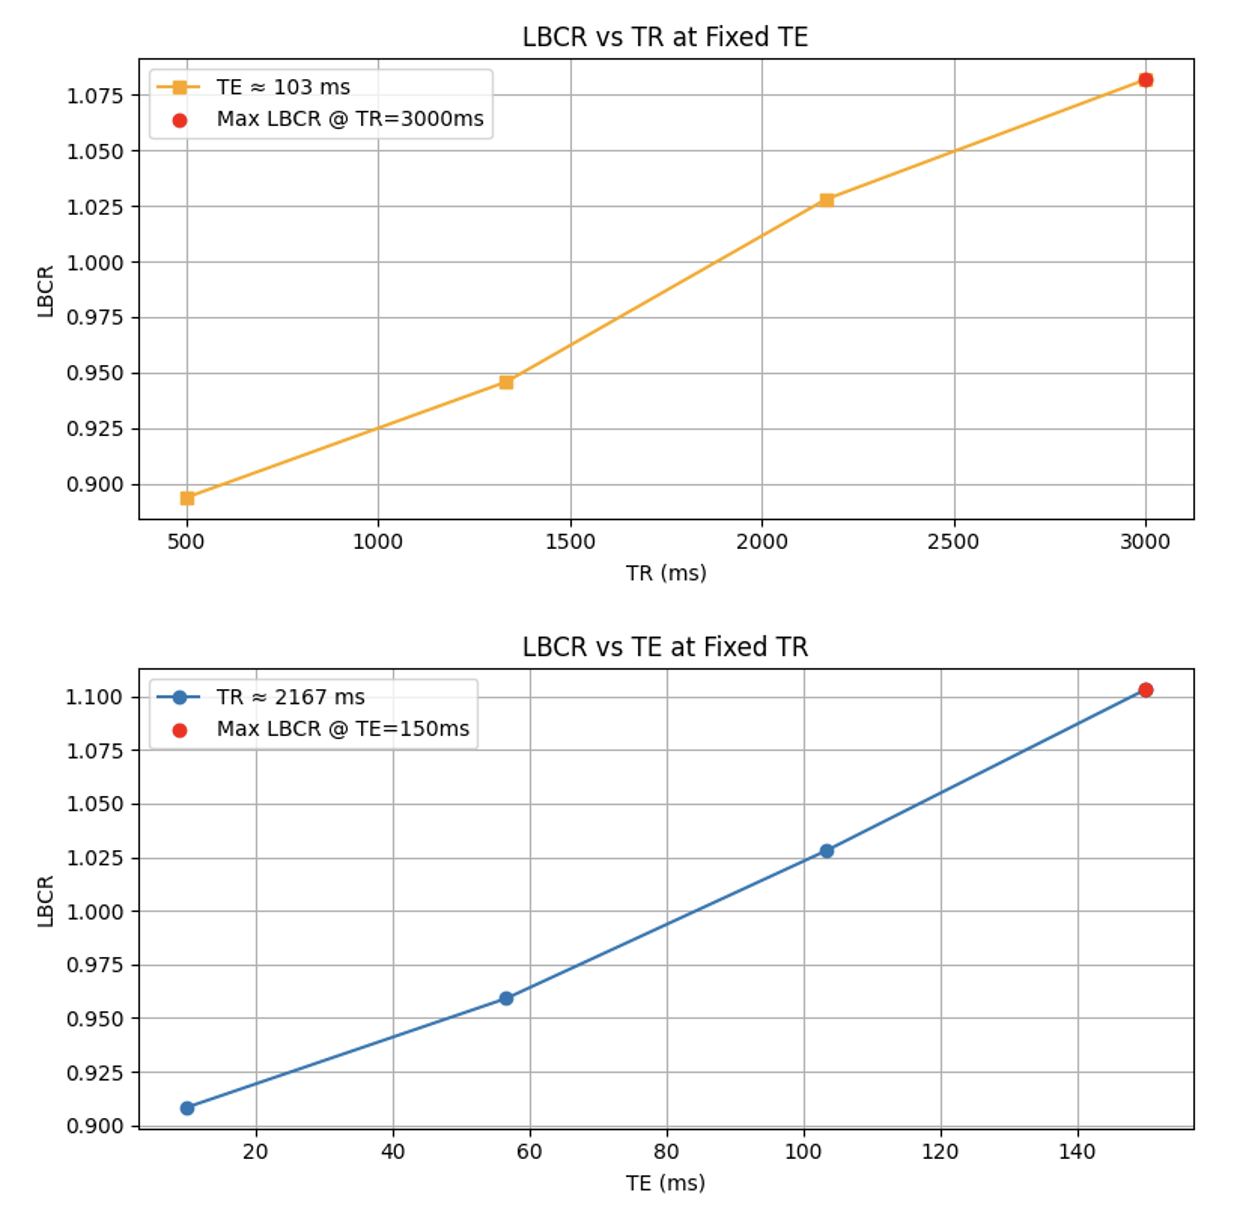
\includegraphics[width=0.9\textwidth]{lbcrslices.png}
\caption{Top: LBCR vs \( T_E \) at fixed \( T_R \) ms; Bottom: LBCR vs \( T_R \) at fixed \( T_E \) ms.}
\label{fig:lbcrslice}
\end{figure}

\subsection{Synthesis}

The findings address the core problem posed in this study: how do spatially varying relaxation parameters within tissues influence MRI signal formation and contrast optimization? Through simulations incorporating voxel-wise \( T_1 \) and \( T_2 \) maps, we demonstrate that contrast behavior is highly sensitive to acquisition settings and intra-lesional heterogeneity. The results affirm past work on signal modeling under relaxation variability \cite{tofts2003, stanisz2005} while extending it to LBCR-based contrast optimization—a less explored metric for simulation-based contrast tuning \cite{naganawa2002}.

Importantly, the LBCR contrast surface suggests a tractable strategy for optimizing imaging parameters without relying solely on empirical testing. As clinical MRI moves toward greater quantification and reproducibility, simulations such as those in this study can guide protocol selection, especially for challenging tissues with non-uniform relaxation properties.






% Please use the style file spp-bst.bst. If you wish to use BibTeX, kindly use us the filename bibfile.bib for your bib file.
\bibliographystyle{spp-bst}
\bibliography{bibfile}

\end{document}